\chapter{Reinforcement Learning}
\label{chapter2}
\thispagestyle{empty}

\begin{quotation}
{\footnotesize
\noindent{\emph{All models are wrong, but some are useful. \\ 
} }
\begin{flushright}
George E. P. Box
\end{flushright}
}
\end{quotation}
\vspace{0.5cm}

\noindent In this chapter, we present the basics of the Reinforcement Learning framework needed for contextualize the work of the following chapters. We will first introduce the Markov Decision Process model, \cref{sec:MDP}, then we present the main approaches for the \textit{exact} solution of Markov Decision Processes, namely \textit{Linear Programming}, \cref{sec:lin_prog}, and \textit{Dynamic Programming}, \cref{sec:dyn_prog}. In \cref{sec:policy-search} we present \textit{Policy Search} algorithms, that represents an approximate solution to the Markov Decision Processes problem. At the end of this chapter we will consider some notable extensions to the Markov Decision Process framework, \cref{sec:mdp-ext}.
\section{Markov Decision Processes} \label{sec:MDP}
% Informal introduction to MDP
A Markov Decision Process \citep{puterman2014markov} (MDP) is a formal framework for modelling sequential decision making problems. The decision maker is usually called \textit{agent}.
 In MDPs an agent interacts with an \textit{environment} through \textit{actions} and receives a \textit{reward} based on the action and on the current state of the environment. The goal of the agent is to maximize the cumulative sum, possibly discounted, of rewards in a given \textit{horizon} (possibly infinite). The task the agent has to learn is defined through the rewards it receives. 
 \subsection{Formal Model}
 %  Formal introduction to MDP
In this work we consider finite-time MDPs in which time is divided in discrete steps. At each time step $t = 0,1,...,H$ the agent receives a representation $s_t$ of the state of the environment, $s_t \in \mathcal{S}$, takes an action, $a_t \in \mathcal{A}$, receives a reward, $r_t \in \mathbb{R}$, and lands in the next state $s_{t+1}$ according to the environment dynamics $P: \mathcal{S} \times \mathcal{A} \rightarrow \Delta(\mathcal{S})$. Here $H$ denotes the horizon length, $H \in \mathbb{R}^+ \cup \{+\infty \} $.\newline
Formally an MDP is a tuple $\langle\mathcal{S}, \mathcal{A}, R, \gamma, P, \mu\rangle$, where:
\begin{itemize}
\item $\mathcal{S}$ is  the \textit{state space} (discrete or continuous);
\item $\mathcal{A}$ is the \textit{action space}  (discrete or continuous);
\item $R : \mathcal{S} \times \mathcal{A} \times \mathcal{S} \rightarrow \mathbb{R}$ is the \textit{reward function};
\item $\gamma \in [0,1]$ is the \textit{discount factor} for future rewards;
\item $P: \mathcal{S} \times \mathcal{A} \rightarrow \Delta (\mathcal{S})$ is the \textit{transition function}, where $P(\cdot | s, a)$ is the probability distribution over the next states given that the agent executes action $a$ in state $s$;
\item $\mu \in \Delta(\mathcal{S}) $ is the initial state distribution.
\end{itemize}

Formally the reward function is defined over $\mathcal{S} \times \mathcal{A} \times \mathcal{S} $, so a reward realization is \newline $R(s_t,a_t,s_{t+1})$. Usually we forget the dependence on the state $s_{t+1}$ by taking the expectation over the next states according to the environment dynamics:
\begin{equation}
	r(s_t,a_t) = \underset{s_{t+1} \sim P(\cdot | s_t, a_t)}{\mathbb{E}} \left[R(s_t,a_t,s_{t+1})\right] .
\end{equation}
A trajectory is sequence $\tau=\langle s_t, a_t, R_t\rangle_{t=0,...,H}$ in which $s_t$ represent the current state, $a_t$ the action taken, $R_t$ the reward received at time step $t$.
\begin{figure}[tb!]
\centering
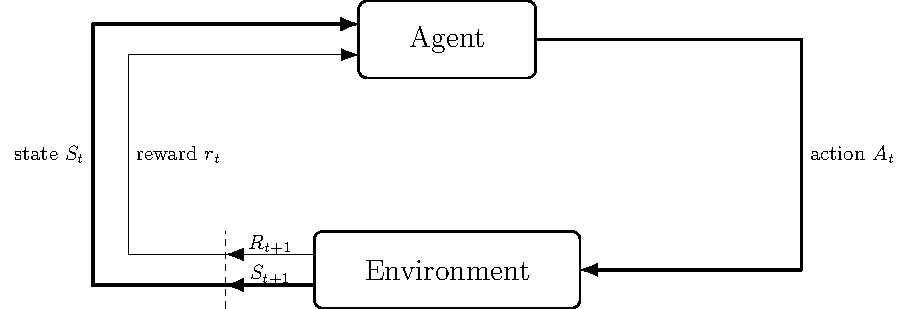
\includegraphics[width=0.8\textwidth]{pictures/agentenv}
\caption{\small Agent Environment interface, from \citep{sutton_introduction}.}
\end{figure}

 \subsection{Transition Model}
 % talk about transition model properties
The transition function must satisfy two properties in order for the problem to be an MDP:
\begin{description}
\item \textit{Markovian}: the current state and action are a sufficient statistic to define the probability over the next states;%Formally the Markovian property states that:
%\begin{equation}
%P(\cdot | s_t, a_t) = P( \cdot | s_t,a_t, s_{t-1}, a_{t-1} ..., s_0, a_0)
%\end{equation}.
\item \textit{Stationarity}: the environment dynamics does not change over time. %, this means that, if $s_{t_1} = s_{t_2}$ and $a_{t_1} = a_{t_2}$, then:
%\begin{equation}
%P(\cdot | s_{t_1}, a_{t_1}) = P( \cdot | s_{t_2},a_{t_2})
%\end{equation}.
\end{description}
These usually are assumptions made in order to simplify the problem. The Markovian property can be ensured by adding enough information to the state. The Stationarity property can be ensured in a similar way, if a task is non stationary it can be translated in a stationary task by adding the time component  to the state description.

 \subsection{Policy} \label{sec:policy}
 % talk about policy properties
The agent interacts with the environment by means of a \textit{policy} that defines its \textit{behaviour}. At each decision epoch a decision maker takes action according to its behaviour $b$. In the most general case the action $a_t$ depends on the whole history from time 0 to time $t$. We denote the set of histories with $\mathbb{H}_t$. A \textit{stochastic} behaviour $b_t$ can be defined as:
\begin{equation}
	b_t : \mathbb{H}_t \rightarrow \Delta(\mathcal{A}) \, .
\end{equation}
A behaviour is said to be \textit{Markovian} if the distribution over actions depends only on the current state:
\begin{equation}
	b_t : \mathcal{S} \rightarrow \Delta(\mathcal{A}) \, .
\end{equation}
A policy is \textit{stationary} if the distribution over actions does not depends on the time.
In this work we will denote a \textit{stationary} \textit{Markovian} policy with $\pi$: 
\begin{equation}
	\pi : \mathcal{S} \rightarrow \Delta (\mathcal{A}) \, .
\end{equation}
It is useful to consider \textit{parameterized} policies, where $\boldsymbol{\theta} \in \mathbb{R}^d$ is the vector of policy parameters. To denote a parameterized policy we use the notation $\pi_{\boldsymbol{\theta}}$ and we omit the subscript when it is clear from the context that the  considered policy is parameterized. The usage of a parameterization implicitly defines a set of policy in which we are interested, we denote the policy family with $\Pi$ and we have $\pi \in \Pi$. 
Common policy parameterizations are:
\begin{description}
\item \textit{Linear} (deterministic), the resulting action is a linear combination of the state features $\phi(s)$:
\begin{equation}
\pi(s) = \boldsymbol{\theta}^T \boldsymbol{\phi}(s) .
\end{equation}
\item \textit{Gaussian}, the resulting action has a gaussian distribution, in which the mean and the variance depend on state features:
\begin{equation}
\pi( \cdot | s) \sim \mathcal{N} ( m( \boldsymbol{\phi}(s)), v(\boldsymbol{\phi}(s)) ) .
\end{equation}
The Gaussian parameterization is useful for continuous action spaces.
\item \textit{Boltzmann}, used for discrete action spaces, the resulting action is a soft-max acting on the weighted state features:
\begin{equation}
\pi(a_i | s) = \frac{e^{\boldsymbol{\theta}_i^T \boldsymbol{\phi}(s)}}{\sum_j e^{\boldsymbol{\theta}_j^T \boldsymbol{\phi}(s)}} \, ,
\end{equation}
where $\boldsymbol{\theta}_i$ is the set of parameters associated to action $a_i$.
\end{description}
In all of these parametrizations the state features might be non-linear features depending on some parameters, e.g. coming from a neural network; radial basis function (RBF) features, tile coding features.

%%%%%%%%%%%%%%%%%% STATE DISTRIBUTION %%%%%%%%%%%%%%%%%%%
\subsection{State distribution} \label{sec:state-distr}
Behaving accordingly to a policy in an MDP induces a distribution over the state space. Here we recall the formulation of the $\gamma$-discounted future state occupancy \citep{pol_grad_func_approx}:
\begin{equation}
	\hat{d}_{\mu,\gamma}^\pi(s) = \sum_{t=0}^{+\infty}\gamma^t \mathbb{P}(s_t = s | \mu, P, \pi) \, .
\end{equation}
The previous formula defines $\hat{d}_\mu^\pi$ of a state $s$ as the sum of the discounted probability of being in $s$ in a time step $t$ given the policy, the initial state distribution and the transition model.
Formally $\hat{d}_\mu^\pi$ is not a distribution as it does not sum up to 1. We normalize it obtaining the $\gamma$ discounted state distribution:
\begin{equation}
	d_{\mu,\gamma}^\pi(s) = (1 - \gamma) \hat{d}_\mu^\pi(s) \, .
\end{equation}
%%%%%%%%%%%%%%%%%% STATE KERNEL %%%%%%%%%%%%%%%%%%%
\subsection{State Kernel}
The transition model and the policy naturally define the \textit{state kernel}, that has a primary role in our work. Formally the state kernel is a function $P^\pi : \mathcal{S} \rightarrow \Delta(\mathcal{S})$. It defines, for each state, a probability measures over the set of states. It consider jointly the effect of the transition model and the policy.
The state kernel is obtained by marginalizing the transition model over the actions:
\begin{equation}
	P^\pi (s' | s) = \int_\mathcal{A} \pi(a | s) P(s' | s, a) \mathrm{d}a \, .
\end{equation}  
%%%%%%%%%%%%%%%%%%%%%%%%%% GOALS and REWARD %%%%%%%%%%%%%%%%%%%
 \subsection{Goal and Rewards}
 % talk about performance objectives, like average reward setting, full return etc
 In Reinforcement Learning the agent's goal is to maximize the total amount of rewards it receives. This is based on the reward hypothesis \citep{sutton_introduction}:
 	
\begin{quotation}
	 \emph{That all of what we mean by goals and purposes can be well thought of as the maximization of the expected value of the cumulative sum of a received scalar signal (called reward).}
\end{quotation}

 Even if a scalar reward signal might seem limiting, this concept has proven to be very flexible and applicable to a wide range of tasks. For example, in locomotion tasks the reward can be defined to be proportional to the amount of distance traveled from the previous step to the current step. In making a robot reaching a goal the reward can be defined as -1 for every step until the agent finds the goal, encouraging the agent to reach the goal as fast as possible.
 It is very important in RL that the reward is given in such a way that it describes what is the goal of the task, it should not describe how to do something. However, in some cases the reward definition might be not trivial. Think for example to a reward for a driving task. In the case of driving it is not trivial to define what does it mean to drive in a good way. \newline
RL tasks can be divided in \textit{episodic} and \textit{continuing}. In episodic tasks we have that $H$, the horizon length, is finite, while in continuing tasks $H = +\infty$.
The \textit{return}, $G_t$ quantifies the agent performance. For \textit{episodic} tasks the return from time step $t$ can be defined as the sum of rewards received until the end of the episode:
\begin{equation}
G_t = \sum_{k=t}^H r_k	\, .
\end{equation}
It is easy to see that for \textit{continuing tasks} this formulation of return diverges since we have an infinite sum of rewards.
To deal with \textit{continuing tasks} we need to introduce the notion of \textit{discounting}. The \textit{discount factor} $\gamma \in [0,1]$ quantifies the present values of future payoffs. 
We introduce the \textit{discounted return} as the cumulative, discounted, sum of rewards until the end of the episode:
\begin{equation}
G_t = \sum_{k=0}^H \gamma^k r_{t+k+1} \, .
\end{equation}
The discount factor, besides having the interpretation mentioned before, can be seen as the probability that the process continues for another step. From the agent point of view, if the discount factor is near to zero greedy actions are profitable since future rewards do not have high values. If the discount factor is near to 1 the agent is \textit{far-sighted}, it is possible for him to sacrifice an action related to a good immediate reward now for a higher reward in the future steps.
We indicate with $G(\tau)$ the return associated with the trajectory $\tau$.
\subsection{Policy and Value Functions}
Policy evaluation is the process of quantifying how good a policy is, it is a key step in almost all RL algorithms. The performance of a policy is defined as the expected value of the return under state and action distribution:
\begin{equation}
J^\pi = \underset{\begin{subarray}{c}
	s_0 \sim \mu \\
	a_t \sim \pi(\cdot | s_t) \\
	s_{t+1} \sim P(\cdot | s_t, a_t)
\end{subarray}
}{\mathbb{E}}\left[ \sum_{t=0}^H \gamma^t R(s_t,a_t, s_{t+1})\right] \, .
\end{equation}
The simple idea formalized above is that policy $\pi_1$ it is better then policy $\pi_2$ if, on average, it collects more rewards. 
Solving an MDP means to find the policy $\pi^*$ such that:
\begin{equation}
\pi^* \in \arg \max_{\pi} J^{\pi} \, .
\label{argmaxJ}
\end{equation}
When we have a parametrized policy we can cast the problem to the point of view of policy parameters. We have that $J$ depends on the policy parameters:
 
\begin{align}
J(\boldsymbol{\theta}) &= \underset{
\begin{subarray}{c}
s_0 \sim \mu \\
	a_t \sim \pi_\theta(\cdot | s_t) \\
	s_{t+1} \sim P(\cdot | s_t, a_t)
\end{subarray}
}{\mathbb{E}}\left[ \sum_{t=0}^H \gamma^{t} R(s_t, a_t, s_{t+1}) \right] . \\
\boldsymbol{\theta}^* & \in \arg \max_{\boldsymbol{\theta}} J(\boldsymbol{\theta}) \, .
\end{align}
The \textit{Value function} (or state-value function) provides a utility measure to a state following a policy. The value of a state $s$ under policy $\pi$, denoted as $v^\pi(s)$, is the expected  discounted return starting from $s$ following the behaviour prescribed by $\pi$:
\begin{equation}
v^\pi(s) = \underset{\pi}{\mathbb{E}} \left[ G_t | s_t = s \right] \, .
\end{equation}
In this way the value function embeds long-term information.
Similarly, we define the value of a state-action pair $(s,a)$ under policy $\pi$ as the expected discounted return starting from $s$, executing action $a$ and following the behaviour $\pi$. This utility measure is denoted as \textit{Q-function} or \textit{action-value function}:
 \begin{equation}
q^\pi(s,a) = \underset{\pi}{\mathbb{E}} \left[ G_t | s_t = s, a_t = a \right] \, .
\end{equation}
 
 The \textit{value function} is not suitable for control as it does not provide information on which action to take. The \textit{Q-function} provides a utility to all actions in a particular state.
 Value function and Q-function are clearly strictly related, the former is obtained by averaging the latter over the action distribution defined by the policy:

 \begin{equation}
v^\pi(s) = \underset{a \sim \pi(\cdot | s)}{\mathbb{E}} \left[ q^\pi(s,a) \right] \, .
\end{equation}

Using the state value function it is possible to re-write the performance of a policy:
\begin{equation}
J^\pi = \underset{s \sim \mu}{\mathbb{E}} \left[ v^\pi(s) \right] \, .
\end{equation}

The value function has also a recursive formulation, denoted as \textit{Bellman expectation operator for $v^\pi$} \citep{Bellman:1957}:
 \begin{equation}
v^\pi(s) = \underset{\begin{subarray}{c}
   a \sim \pi(\cdot | s) \\
   s'\sim P(\cdot | s,a)
   \end{subarray}}
   {\mathbb{E}} \left[R(s,a,s') + \gamma v^\pi (s') \right] \, .
\end{equation}
We can express in a recursive manner also the Q-function, the associated operator is denoted as \textit{Bellman expectation operator for $q^\pi$}:
 \begin{equation}
q^\pi(s,a) = \underset{\begin{subarray}{c}
   a' \sim \pi(\cdot | s') \\
   s' \sim P(\cdot | s,a)
   \end{subarray}}
   {\mathbb{E}} \left[R(s,a,s') + \gamma q^\pi(s',a')\right] \, .
\end{equation}

The Bellman expectation operators have several properties (see \ref{sec:opt-cond}). The operators are mainly used in iterative policy evaluation (see \ref{sec:pi}). We give the formal definition of the Bellman Expectation operators.
%%%%%%%%%%%%%%%%%%% BELLMAN EXPECTATION OPERATOR %%%%%%%%%%%%%%%%%%%%%%
\begin{definition}[Bellman Expectation Operator for $v^\pi$]
	The Bellman expectation operator for $v^\pi$ is defined as $T^{\pi} : \mathbb{R}^{| \mathcal{S} |} \rightarrow \mathbb{R}^{| \mathcal{S} | }$, maps state-value functions to state-value functions:
	\begin{equation}
		(T^{\pi} v)(s) = \underset{\begin{subarray}{c}a \sim \pi(s) \\ s' \sim P(\cdot | s,a) \end{subarray}}{\mathbb{E}} \left[ R(s,a,s') + \gamma v(s') \right] \, .
	\end{equation}
\end{definition} \label{def:bellman_exp_op_for_v}
\begin{definition}[Bellman Expectation Operator for $q^{\pi}$]
	The Bellman expectation operator for $q^{\pi}$ is defined as $T^{\pi} : \mathbb{R}^{| \mathcal{S} | \times | \mathcal{A} |} \rightarrow \mathbb{R}^{| \mathcal{S} | \times | \mathcal{A} |}$, maps Q-functions to Q-functions:
	\begin{equation}
		(T^{\pi} q)(s,a) =\underset{\begin{subarray}{c} a' \sim \pi(s') \\ s' \sim P(\cdot | s,a) \end{subarray}}{
			\mathbb{E}} \left[ R(s,a,s') + \gamma q(s',a') \right] \, .
	\end{equation}
\end{definition} \label{def:bellman_exp_op_for_q}


%%%%%%%%%%%%%%%% OPTIMALITY CONDITIONS %%%%%%%%%%%%%%%%%%5
\subsection{Optimality Conditions}\label{sec:opt-cond}
Besides \cref{argmaxJ} we can define another partial ordering over policies, the ordering induced by \textit{value functions}.
\begin{definition}
\label{optimal_policy}
	Policy $\pi$ is better or equal ($\succeq$) policy $\pi'$ if its expected return is greater or equal to that of $\pi'$ \textit{for all states}:
	\begin{equation}
		\pi \succeq \pi' \iff v^\pi(s) \geq v^{\pi'}(s), \; \forall s \in \mathcal{S} \, .
	\end{equation}
\end{definition}  

Following the previous definition an \textit{optimal policy} is a policy that is better or equal to all other policies in all states. This optimality condition is stricter than the one presented in (\ref{argmaxJ}).
From the definition of optimal policy the \textit{optimal state-value function} and the \textit{optimal Q-function} follows:
\begin{align}
	v^{*}(s) &= \max_\pi v^\pi(s) \\
	q^{*}(s,a) &= \max_\pi q^\pi(s,a) \, .
\end{align}
There is always at least an optimal (deterministic) policy maximizing the state-value function in every state \citep{Puterman:1994:MDP:528623} and all optimal policies share the same \textit{optimal state value-function}. 
The knowledge of the \textit{optimal} Q-function makes it possible to find the \textit{optimal} deterministic policy selecting in every state the action yielding the highest $q$-value: 
\begin{equation}
	\pi^*(s) \in \arg \max_a q^{*}(s,a) \, .
\end{equation}

This holds if we have complete freedom in the selection of the policy (i.e. when $\Pi$ is the set of all Markovian policies). However for practical algorithms we need to restrict our policy space (e.g. parametric policy space), in these cases it is convenient to use the definition of optimal policy in (\ref{argmaxJ}). 
\newline
The optimal state-value function and optimal Q-function satisfy the \textit{Bellman optimality equations}:
\begin{align}
	v^*(s) &= \max_a q^*(s,a) \label{opt_v} \\
		   &= \max_a \underset{s' \sim P(\cdot | s,a)}{
			\mathbb{E}} \left[ R(s,a,s') + \gamma v^*(s') \right] \, . \\			
	q^*(s,a) &= \underset{s' \sim P(\cdot | s,a)}{
			\mathbb{E}} \left[ R(s,a,s') + \gamma \max_{a'} q^*(s',a') \right] \label{opt_q} \, .
\end{align}
At an intuitive level the \textit{Bellman optimality equation} for $v^*$ expresses the fact that the optimal state-value function must equal the expected return for the best action in that state. The \textit{Bellman optimality equation} for $q^*$, similarly, expresses the fact that the optimal Q-function must equal the immediate reward plus the discounted return of the best action in the next state according to the environment dynamic. \newline
The right handside of \cref{opt_v} it's defined as \textit{Bellman Optimality Operator}.

%%%%%%%%%%%%%%%%%%% BELLMAN OPTIMALITY OPERATOR %%%%%%%%%%%%%%%%%%%%%%
\begin{definition}[Bellman Optimality Operator for $v^*$]
	The Bellman optimality operator for $v^*$ is defined as $T^* : \mathbb{R}^{| \mathcal{S} |} \rightarrow \mathbb{R}^{| \mathcal{S} | }$, maps state-value functions to state-value functions:
	\begin{equation}
		(T^* v)(s) = \max_a \underset{s' \sim P(\cdot | s,a)}{\mathbb{E}} \left[ R(s,a,s') + \gamma v(s') \right] \, .
	\end{equation}
\end{definition} \label{def:bellman_opt_op_for_v}
\begin{definition}[Bellman Optimality Operator for $q^*$]
	The Bellman optimality operator for $q^*$ is defined as $T^* : \mathbb{R}^{| \mathcal{S} | \times | \mathcal{A} |} \rightarrow \mathbb{R}^{| \mathcal{S} | \times | \mathcal{A} |}$, maps Q-functions to Q-functions:
	\begin{equation}
		(T^* q)(s,a) =\underset{s' \sim P(\cdot | s,a)}{
			\mathbb{E}} \left[ R(s,a,s') + \gamma \max_{a'} q(s',a') \right] \, .
	\end{equation}
\end{definition} \label{def:bellman_exp_op_for_v}
The Bellman operators (\ref{def:bellman_exp_op_for_v}, \ref{def:bellman_exp_op_for_q}, \ref{def:bellman_opt_op_for_v}, \ref{def:bellman_exp_op_for_q}) are characterized by the following properties, where we will use $T$ to denote both the expectation operator and the optimality operator:
\begin{itemize}
	\item Monotonicity: \begin{equation}
			f_1 \leq f_2 \implies T f_1 \leq T f_2 \, ;
		\end{equation}
	\item Max-Norm contraction:
			\begin{equation}
			\norm{T f_1 - T f_1}_\infty \leq \gamma \norm{f_1 - f_2}_\infty \, , \forall f_1, f_2 \, ;
		\end{equation}
	\item $v^*$ is the \textit{unique fixed point} of $T^*$. $v^\pi$ is the \textit{unique fixed point} of $T^{\pi}$.
	\item Convergence: 
	 \begin{equation}
			\lim_{k \rightarrow \infty} (T^*)^k f = v^* \, , \forall f \in \mathbb{R}^{| \mathcal{S} |} \, 
		\end{equation}
		\begin{equation}
			\lim_{k \rightarrow \infty} (T^{\pi})^k f = v^\pi \, , \forall f \in \mathbb{R}^{| \mathcal{S} |} \, .
		\end{equation}
\end{itemize}
Solving \cref{opt_v} and \cref{opt_q} leads us directly to the MDP solution. Unfortunately these equations are non-linear because of the presence of the $\max$ operator and there is no closed form solution for the general case. 
There exists many iterative solution methods trying to solve an approximation of the Bellman optimality equations that are discussed in the following sections.

\section{Linear Programming} \label{sec:lin_prog}
The problem of computing an optimal policy for an infinite horizon finite-states MDP can be formulated as linear program (LP) \citep{depenoux_probabilistic_1963}. In this section we will go further in the LP formulation since our algorithm extends on this.
The basic idea follows from \cref{optimal_policy}: we want to find the value function maximizing the value of each state weighted by the initial state distribution subject to a feasibility constraint:
\begin{align*}
	\underset{v}{\text{minimize}} & \; \sum_{s \in \mathcal{S}} \mu(s) v(s) \\
	\text{subject to} &  \; v(s) \geq r(s,a) + \gamma \sum_{s' \in \mathcal{S}} P(s' | s,a) v(s') \, , \forall s \in \mathcal{S}, \, \forall a \in \mathcal{A} \, .
\end{align*} 
Where we have $|\mathcal{S}|$ variables and $|\mathcal{S}| |\mathcal{A}|$ constraints. Notice that the maximization role is taken by the constraints, while we need to minimize since otherwise an optimal solution would have infinite values for all variables $v$.
\begin{theorem}[Linear Programming Solution]
$v^*$ is the solution of the above linear program.
\end{theorem} \label{lpth}	


It is possible to prove the above theorem using the properties of the Bellman optimality operators, the interested reader can refer to \cref{LPproof}.
It is also interesting to analyze the Dual Linear Program:

\begin{align*}
	\underset{p}{\text{maximize}} & \; \sum_{s \in \mathcal{S}} \sum_{a \in \mathcal{A}} d(s,a)r(s,a) \\
	\text{subject to} &  \; \sum_{a \in \mathcal{A}} d(s,a) = \mu(s) + \gamma \sum_{s' \in \mathcal{S}} \sum_{a' \in \mathcal{A}} d(s',a') P(s | s', a'), \; \forall s \in \mathcal{S} \\
	& d(s,a) \geq 0, \;  \forall s \in \mathcal{S}, \; \forall a \in \mathcal{S} \, .
\end{align*} 

In the dual program $d(s,a)$ is the discounted state action distribution \citep{pol_grad_func_approx}:
\begin{equation}
	d(s,a) = \sum_t^\infty \gamma^t \mathbb{P}(s_t = s, a_t = a) \, .
\end{equation}

The objective of the dual is the usual objective: maximize the expected discounted sum of rewards.
The constraints are needed for ensuring that $p$ is a valid distribution. 
From the dual program it is possible to extract the optimal policy:
\begin{equation}
	\pi^*(s) \in \arg \max_a d(s,a)\, .
\end{equation}
For each state $s$ we have that $d(s,a^*) = 1$ if action $a^*$ is optimal in state $s$. When there are multiple optimal actions we have a split of the probability between these actions.
The LP formulation is an exact way of solving the MDPs, unfortunately this formulation becomes impractical when the states space grows too much.

\section{Dynamic Programming} \label{sec:dyn_prog}
Dynamic programming \citep{Bellman:1957} (DP) is by far the most common way for solving MDPs when the dynamics and the reward function are known. DP takes into account the sequential or temporal structure of the problem. It is a method for solving complex problems by breaking them into subproblems.
A problem, in order to be solved by DP techniques, must have two properties: \begin{enumerate*} \item Optimal Substructure, \item Overlapping Subproblems \end{enumerate*}. The optimal substructure property means that the principle of optimality applies and the optimal solution can be decomposed into subproblems. The overlapping subproblems property means that subproblems recur many times and the solutions can be stored and reused.
In MDPs both properties are satisfied. The \textbf{Bellman equation} gives the recursive decomposition while the \textbf{state-value function} caches and reuses previous solutions.

\begin{figure}[tb]
\centering
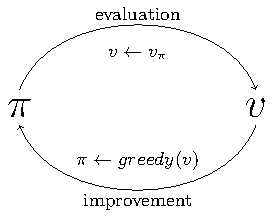
\includegraphics{pictures/value_iteration}
\caption{\small Policy Iteration, from \citep{sutton_introduction}.}
\end{figure}

\subsection{Policy Iteration} \label{sec:pi}
Policy Iteration \citep{howard:dp} is a two stage algorithm: Policy Evaluation (PE) and Policy Improvement (PI).
The first stage (Policy Evaluation) aims at evaluating the current policy through the application of the Bellman Expectation Operator. The PE phase is needed since we want to perform an update of the current policy. The update direction can be computed using the action-value function in the following way. Suppose we know $v^\pi(s')$ for a particular $s'$. To improve the current policy it is enough to compute $q^\pi(s',a)$ for each $a \in \mathcal{A}$ and then to compare it with $v^\pi(s')$. If exists an action $a'$ such that $q(s',a') > v^\pi(s')$, then we can \textit{improve} the current policy using the following update rule:
\begin{equation}
\pi'(s) =
	\left\{
	\begin{array}{ll}
		\pi(s)  & \mbox{if } s \neq s' \\
		\underset{a}{\arg \max} \, q^\pi(s,a) & \mbox{if } s = s'
	\end{array}
\right .
\label{eq:greedy1}
\end{equation}
Basically this update rule states that the new policy is the same as the old policy except for states in which there exists an action $a$ such that the action-value function $q^\pi$ is greater than the value function $v^\pi$. 
The justification for the previous statement comes from the \textit{Policy Improvement Theorem}.
\begin{theorem}[Policy Improvement Theorem]
	Let $\pi$ and $\pi'$ be a pair of policies such that:
	\begin{equation}
		q^\pi(s, \pi'(s)) \geq v^\pi(s) \, , \forall s \in \mathcal{S} \, ,
	\end{equation}
	Then the policy $\pi'$ must be as good or better than $\pi$. 
	\label{th:policy_improvement}
\end{theorem}

Given the previous theorem we can expand the update rule (\ref{eq:greedy1}) by computing the \textit{greedy policy} in all states:
\begin{equation}
\pi'(s) \in \underset{a}{\arg \max} \, q^\pi(s,a) 	\, .
	\label{eq:greedy2}
\end{equation}

This update rule meets the condition of \cref{th:policy_improvement}, so the updated policy is as good as, or better than the old one. 
When the new policy is as good as the old, $v^{\pi'} = v^\pi$, we know, thanks to the optimality operator property, that $v^\pi = v^*$, we have obtained the optimal policy.
Now we can formalize the Policy Iteration Algorithm, see \cref{alg:policy-iteration}.
All the previous ideas can be easily extended to the case of stochastic policies.

\begin{algorithm}[tb]
  \caption{Policy Iteration
    \label{alg:policy-iteration}}
  \begin{algorithmic}[1]
  \Require{$\mathcal{S}, \mathcal{A}, P, R$}
  \Ensure{$\pi \approx \pi^*$}
  \State Initialize $v^\pi$ and $\pi$ randomly
  \Repeat
  \State $v^\pi$ $\leftarrow$ Evaluate policy $\pi$ by applying $T^{\pi}$
  \State $\pi$ $\leftarrow$  Improve policy $\pi$
  \Until{no improvement found} \\
  \Return{Policy $\pi$} 	
  \end{algorithmic}
\end{algorithm}

\subsection{Value Iteration}  
The Value Iteration (VI) algorithm performs evaluation and improvement in the same step. While Policy Iteration performs a search in the space of policies, Value Iteration searches in the space of value functions, calculating the policy only in the last step.
Value Iteration is obtained simply by turning the Bellman Optimality Operator into an update rule:
\begin{equation}
		v_{k+1}(s) = \max_a \underset{s' \sim P(\cdot | s,a)}{\mathbb{E}} \left[ R(s,a,s') + \gamma v_{k}(s') \right] \, , \forall s \in \mathcal{S} \, .
\end{equation}
Value Iteration algorithm is reported in \cref{alg:value-iteration}. \newline
Both PI and VI converge to an optimal policy for discounted finite MDPs.

\begin{algorithm}[tb]
  \caption{Value Iteration
    \label{alg:value-iteration}}
  \begin{algorithmic}[1]
  \Require{$\mathcal{S}, \mathcal{A}, P, R$}
  \Ensure{$\pi \approx \pi^*$}
  \State Initialize $v$ randomly
  \Repeat
  \State $v$ $\leftarrow$ Apply Bellman Optimality operator $T^*v$
  \Until{no changes in the value function} \\
  \Return{Policy $\pi$:
  \begin{equation}
  	\pi(s) = \underset{a}{\arg \max} \underset{s' \sim P(\cdot | s,a)}{\mathbb{E}} \left[ R(s,a,s') + \gamma v(s') \right] \, , \forall s \in \mathcal{S} \, .
  \end{equation}
  } 	
  \end{algorithmic}
\end{algorithm}
\section{Policy Search}\label{sec:policy-search}
Policy search (PS) methods explore directly the policy space. In the PS framework the RL problem is formalized as:
\begin{equation}
	\pi^* \in \arg \max_{\pi \in \Pi} J^\pi \, .
\end{equation}
Among PS methods it is worth mentioning policy gradient methods \citep{pol_grad_func_approx, PETERS2008682}. Policy gradient methods consider a set of parameterized policies (see \cref{sec:policy}) $\pi_{\boldsymbol{\theta}}(a|s)$ where $\boldsymbol{\theta} \in \mathbb{R}^d$ is the vector of policy parameters. In this cases the space of policies is represented by $\Pi = \left\{ \pi_{\boldsymbol{\theta}} : \boldsymbol{\theta} \in \Theta \subseteq \mathbb{R}^d \right\}$.  A standard requirement is that the policy must be differentiable in its parameters.
A common technique to maximize the performance of a policy is to perform \textit{gradient ascent} over the policy parameters:
\begin{equation}
	\boldsymbol{\theta}^{k+1} = \boldsymbol{\theta}^k + \alpha \nabla_{\boldsymbol{\theta}} J(\boldsymbol{\theta}^k) \, ,
	\label{eq:theta-update}
\end{equation}
where $\alpha \geq 0$ is the \textit{learning rate}, also called \textit{step size}. The quantity $\nabla_{\boldsymbol{\theta}} J(\boldsymbol{\theta}^k)$ is the gradient of the performance of the policy and it can be computed through the policy gradient theorem \citep{pol_grad_func_approx}.
\begin{theorem}[Policy Gradient Theorem] For any MDP:
\begin{equation}
	\nabla_{\boldsymbol{\theta}} J(\boldsymbol{\theta}) = \int_\mathcal{S} d_{\mu, \pi_{\boldsymbol{\theta}}}(s)\int_\mathcal{A} \nabla_{\boldsymbol{\theta}}\pi_{\boldsymbol{\theta}}(a | s) q^{\pi_{\boldsymbol{\theta}}}(s,a) da ds \,.
\label{eq:pol-grad}
\end{equation}
\end{theorem} 
In real cases since the state distribution is not known it is not possible to compute analytically the gradient of the performance measure. We need to resort to a sample approximation of it. 
Gradient ascent method guarantees convergence at least to a local optimum even if in practice local optima can be avoided using a stochastic approximation to the gradient or policies belonging to high dimensional spaces.

\subsubsection{Gradient Estimation}
REINFORCE method \citep{reinforce} builds on the fact that the outer integral in \cref{eq:pol-grad} is the analytical expression of the expected value under the state distribution induced by the policy $\pi$. We can rewrite the gradient in the following way (where we use $\pi$ for $\pi_{\boldsymbol{\theta}}$):
\begin{align}
	\nabla_{\boldsymbol{\theta}} J(\boldsymbol{\theta}) &= \underset{s \sim d_{\mu,\pi}(\cdot)}{\mathbb{E}} \left[ \int_\mathcal{A} \nabla \pi(a | s) q^\pi (s,a) ds \right] \\
	& = \underset{\begin{subarray}{c}
					s \sim d_{\mu,\pi}(\cdot) \\
					a \sim \pi(\cdot |s )
				  \end{subarray}}
		{\mathbb{E}} \left[ \nabla \log \pi(a | s) q^\pi(s,a) \right], \tag*{log trick: $\nabla f = f \nabla \log f$} 
\end{align}
The estimation of the action value function can be performed in a straightforward way from the sum of discounted rewards: $\widehat{q}^\pi \approx \sum_{k=0}^H \gamma^k r(s_k,a_k) $
Summarizing, we can obtain an approximation of the gradient through the following estimator:
\begin{equation}
	\widehat{\nabla_\theta J(\boldsymbol{\theta})}_{RF} = \langle \left(\sum_{k=0}^H \nabla_\theta \log \pi(a_k, s_k) \right) \left( \sum_{k=0}^H \gamma^k r(s_k,a_k) \right) \rangle_N \, ,  
\end{equation}
where $N$ is the batch size, the number of collected trajectories, $\langle \cdot \rangle_N$ denotes the sample mean over $N$ trajectories and $H$ is the horizon length. \newline
REINFORCE gradient estimation suffers of high variance, that grows at least cubically with the length of the horizon and quadratically with the magnitude of the reward. \newline
G(PO)MDP \citep{gpomdp} employs a better approximation with lower variance exploiting the observation that future actions do not depend on past rewards (if the policy does not change within an episode) leading to the following estimation:
\begin{equation}
	\widehat{\nabla_\theta J(\boldsymbol{\theta})}_{G(PO)MDP} = \langle \sum_{l=0}^H \left( \sum_{k=l}^H \nabla_\theta \log \pi(a_k | s_k) \right) \left( \gamma^l r(s_l,a_l) \right) \rangle_N \, .
\end{equation}
\subsubsection{Natural Policy Gradient}
As presented in \citep{NIPS2012_4576}, the general form of Policy Gradient updates is:
\begin{equation}
	\boldsymbol{\theta}^{k+1} = \boldsymbol{\theta}^k + \alpha \mathbf{G}(\boldsymbol{\theta}^k)^{-1}\nabla_{\boldsymbol{\theta}} J(\boldsymbol{\theta}^k) \, ,
\end{equation}
 where $\mathbf{G}(\boldsymbol{\theta})$ is a positive definite matrix. The matrix $\mathbf{G}(\boldsymbol{\theta})$ defines the metric used to measure vectors in the parameter space. The parameter update in Equation (\ref{eq:theta-update}) can be derived from this formulation by using $\mathbf{G}(\boldsymbol{\theta}^k)=\boldsymbol{I}$, that is the Euclidean norm. This assumption does not take into account that the space parameterized is actually a Riemannian manifold. As \citep{amari_1998} suggested it is better to define a metric based not on the choice of coordinates but rather on the manifold (i.e. the surface) that these coordinates parameterize. 
 Natural Gradient \citep{kakade_natural_2002} exploits this structure and uses as metric the Fisher Information Matrix of the trajectory distribution and due to the Markovian structure of the dynamics it is given by:
\begin{equation}
	\mathbf{G}(\boldsymbol{\theta}) = \underset{\begin{subarray}{c}
	s \sim d_{\mu,\gamma}^\pi(\cdot) \\
	a \sim \pi_{\boldsymbol{\theta}}(\cdot | s)	
	\end{subarray}
	}{\mathbb{E}} \left[ \nabla_{\boldsymbol{\theta}} \log \pi_{\boldsymbol{\theta}} (a |s) \nabla_{\boldsymbol{\theta}} \log \pi_{\boldsymbol{\theta}} (a |s)^T \right] \, . 
\end{equation}
Convergence to a local maximum is guaranteed; by choosing a more direct path to the optimal solution in parameter space, the natural gradient has faster convergence and avoids premature convergence of steepest ascent gradient; the natural policy gradient can be shown to be covariant, i.e., independent of the parameterization of the policy; it requires fewer data points for a good gradient estimate.

\clearpage


%%%%%%%%%%%%%%%%%% MDP EXTENSIONS %%%%%%%%%%%%%%
\section{MDP extensions}\label{sec:mdp-ext}
The standard MDP framework has been extended in the literature in order to cover many real cases scenarios. Here we report some notable extensions that can be related and compared to the framework considered in this work.



\subsection{MDP with imprecise probability}
MDP with imprecise probability (MDPIP) \citep{harmanec_generalizing_2002} covers the case in which it is not easy (or even possible) to define a precise probability measure for a given transition $P(\cdot | s, a)$. In this cases the probability parameters are imprecise and therefore the transition model cannot be defined by means of a probability distribution but it must be defined through a set of probability distribution. These sets of distribution are known as transition credal sets $\mathcal{K}(\cdot | s,a)$.\newline
In this framework it is common to use game theoretic approaches maximizing the lowest expected reward with respect to the probability parameters, known as $\Gamma$-maximin criterion. In this cases the optimal value function is:
\begin{equation}
	v^*(s) = \max_{a \in \mathcal{A}} \left\{ \min_{P(\cdot | s,a) \in \mathcal{K}(\cdot | s,a)} r(s,a) + \gamma \sum_{s' \in \mathcal{S}} P(s' | s,a)v^*(s') \right\} \, .
\end{equation} 

\subsection{Bounded-parameter Markov decision processes}
Bounded-parameter MDPs \citep{givan_bounded-parameter_2000} can be used to represent variation or uncertainty concerning the parameters of sequential decision problems in cases where no prior probabilities on the parameter values are available. BMDPs form an efficiently solvable special case of the class of MDPIPs.
In this context interval value functions are introduced as a natural extension of traditional value functions. An interval value function assigns a closed real interval to each state, representing the fact that the value of that state falls within that interval. An interval value function can be used to bound the performance of a policy over the set of exact MDPs associated with a given bounded-parameter MDP.
\subsection{Non stationary MDPs}
Non stationary MDPs \citep{bowerman_1974} are used to model scenarios in which the transition dynamic and the reward function are non stationary, i.e. they change over time. We can model this scenario with a different transition and reward functions for each timestep:
\begin{align}
	&P(s' | s, a, t) = P^t(s' | s,a) \\
	&R(s,a,s',t) = R^t(s,a,s') \, .
\end{align}
A usual assumption made in this family of MDPs is that there is a correlation between contniguous time frames. In this way the agent can use recent experience and forget past experience. In \citep{nonstatmdp} an optimality condition for non stationary MDPs has been defined. Moreover, \citep{GARCIA2000304}, \citep{Cheevaprawatdomrong:2007} and \citep{nonstatmdp2} focused on how to find an optimal policy for non stationary MDPs in an effective way.